\documentclass[11pt]{article}
\usepackage[a4paper,margin=1in]{geometry}
\usepackage{graphicx}
\usepackage{booktabs}
\usepackage{caption}
\usepackage{subcaption}
\usepackage{amsmath}
\usepackage{float}
\usepackage{titlesec}
\usepackage{xcolor}
\usepackage{hyperref}
\usepackage{fancyhdr}
\usepackage{array}

\hypersetup{
    colorlinks=true,
    linkcolor=blue!50!black,
    urlcolor=blue!50!black,
    citecolor=blue!50!black
}

\titleformat{\section}{\normalfont\Large\bfseries}{\thesection}{1em}{}
\titleformat{\subsection}{\normalfont\large\bfseries}{\thesubsection}{1em}{}

\pagestyle{fancy}
\fancyhf{}
\fancyhead[L]{Structural and Modal Analysis of a Wheel Rim}
\fancyhead[R]{\thepage}
\renewcommand{\headrulewidth}{0.4pt}

\setlength{\parskip}{0.5em}
\setlength{\parindent}{0pt}

\title{\textbf{Structural and Modal Analysis of a Wheel Rim CAD Model} \\[0.3em]
\large Static Structural (Radial and SAE J328 Bending Load) and \\
Free-Free / Constrained / Tire-Loaded Modal Studies in Ansys Mechanical}
\author{}
\date{}

\begin{document}

\begin{titlepage}
\centering
\vspace*{3cm}
{\Huge\bfseries Structural and Modal Analysis of\\[0.3em] a Wheel Rim CAD Model\par}
\vspace{1cm}
{\Large Static Structural (Radial and SAE J328 Bending Load) and\\
Free-Free / Constrained / Tire-Loaded Modal Studies\\ in Ansys Mechanical\par}
\vspace{2cm}
{\large Finite Element Analysis Project Report\par}
\vspace{0.5cm}
{\large Department of Mechanical Engineering\par}
\vfill
{\large August 21, 2026\par}
\end{titlepage}

\tableofcontents
\newpage

\section{Introduction}

Wheel rims are safety-critical rotating components subject to a wide range of static and
cyclic loads during vehicle operation, as well as dynamic excitation from road roughness,
tire non-uniformity, and rotational imbalance. A thorough structural characterisation of
a wheel therefore requires both a static structural assessment of stress and deformation
under representative loading, and a modal (free-vibration) assessment of its natural
frequencies and mode shapes.

This project presents both types of analysis for a commercially styled multi-spoke wheel
rim, performed in Ansys Mechanical. The rim geometry was designed and modelled in
SolidWorks and subsequently imported into Ansys via SpaceClaim. The report is structured
in two parts:

\begin{itemize}
    \item \textbf{Part I -- Static Structural Analysis:} the rim is analysed under (a) a
    simplified static radial load representing vehicle weight transmitted through the tire
    contact patch, and (b) a bending moment derived from the SAE J328 cornering fatigue
    test standard, which is the industry-standard load case used to qualify wheel designs.
    \item \textbf{Part II -- Modal Analysis:} the rim's natural frequencies and mode
    shapes are studied under free-free, bolt-hole-constrained, and a simplified
    tire-loaded (distributed mass + radial spring) configuration, preceded by a mesh
    convergence study.
\end{itemize}

\subsection{Geometry, Material, and Mesh}

The wheel rim CAD model was imported into Ansys SpaceClaim 2026 R1 as a single, clean
solid body, with no gaps or surface defects detected. The rim was assigned an
\textbf{Aluminium Alloy} material (Table~\ref{tab:material}) consistent with the
356.0-T6 permanent-mold cast aluminium alloy identified in the source CAD file. The same
geometry, material, and a converged mesh (Section~\ref{sec:convergence}) were reused
across all static and modal analyses in this report for consistency.

\begin{table}[H]
\centering
\caption{Material properties used for the wheel rim}
\label{tab:material}
\begin{tabular}{lc}
\toprule
\textbf{Property} & \textbf{Value} \\
\midrule
Density & 2770 kg/m$^3$ \\
Young's Modulus & 71 GPa \\
Poisson's Ratio & 0.33 \\
Tensile Yield Strength & 280 MPa \\
Tensile Ultimate Strength & 310 MPa \\
\bottomrule
\end{tabular}
\end{table}

\begin{center}
{\LARGE\bfseries Part I}\\[0.3em]
{\Large\bfseries Static Structural Analysis}
\end{center}
\vspace{0.5em}

\section{Methodology}

Two static structural load cases were analysed, both using a Fixed Support applied to the
cylindrical faces of the five bolt holes (representing the wheel bolted to a hub), and the
same converged mesh used throughout this report.

\subsection{Case 1: Simplified Radial Load}

A vertical (radial) load of 4000~N was applied at a Remote Point located at the bottom of
the outer flange, representing the ground reaction force transmitted through the tire
contact patch under a typical passenger car corner weight ($\sim$400~kg). The load was
applied as a Remote Force with Deformable behaviour, directed toward the fixed hub.

\subsection{Case 2: SAE J328 Cornering Bending Moment}

To represent a more realistic and structurally demanding loading condition, a bending
moment was applied following the SAE J328 rotating bending fatigue test standard. In the
physical test, the wheel is bolted to a rotating spindle while a stationary arm applies a
constant bending moment at the rim via a bearing, so that every point on the rim cycles
through tension and compression as the wheel rotates. The static configuration analysed
here represents a single instant of that cycle, with the moment applied at the rim's outer
flange edge (same Remote Point location as Case~1) and the hub fixed at the bolt holes.

The bending moment magnitude was calculated using the standard SAE J328 formula:
\begin{equation}
M = W \times R \times \mu \times S
\label{eq:sae}
\end{equation}
where $W = 4000$~N is the static wheel load, $R = 0.30$~m is the assumed tire rolling
radius, $\mu = 1.1$ is the standard simulated cornering friction coefficient, and
$S = 1.5$ is the standard severity/design factor, giving:
\begin{equation}
M = 4000 \times 0.30 \times 1.1 \times 1.5 \approx 2000\ \text{N·m}
\label{eq:sae_value}
\end{equation}

This moment was applied as a Remote Moment at the same Remote Point used for Case~1,
resolved into in-plane components tangential to the wheel's circumference at that
location, so that it produces a genuine bending action about the rim rather than a
simple torque about the wheel axis.

\section{Results}

\subsection{Case 1: Radial Load Results}

\begin{table}[H]
\centering
\caption{Static structural results under 4000~N radial load}
\label{tab:radial_results}
\begin{tabular}{lc}
\toprule
\textbf{Quantity} & \textbf{Value} \\
\midrule
Maximum Equivalent (von-Mises) Stress & 20.9 MPa \\
Maximum Total Deformation & 26.16 $\mu$m \\
Maximum Equivalent Elastic Strain & $2.96 \times 10^{-4}$ m/m \\
Minimum Safety Factor (vs. 280 MPa yield) & 13.4 \\
\bottomrule
\end{tabular}
\end{table}

\begin{figure}[H]
\centering
\begin{subfigure}{0.48\textwidth}
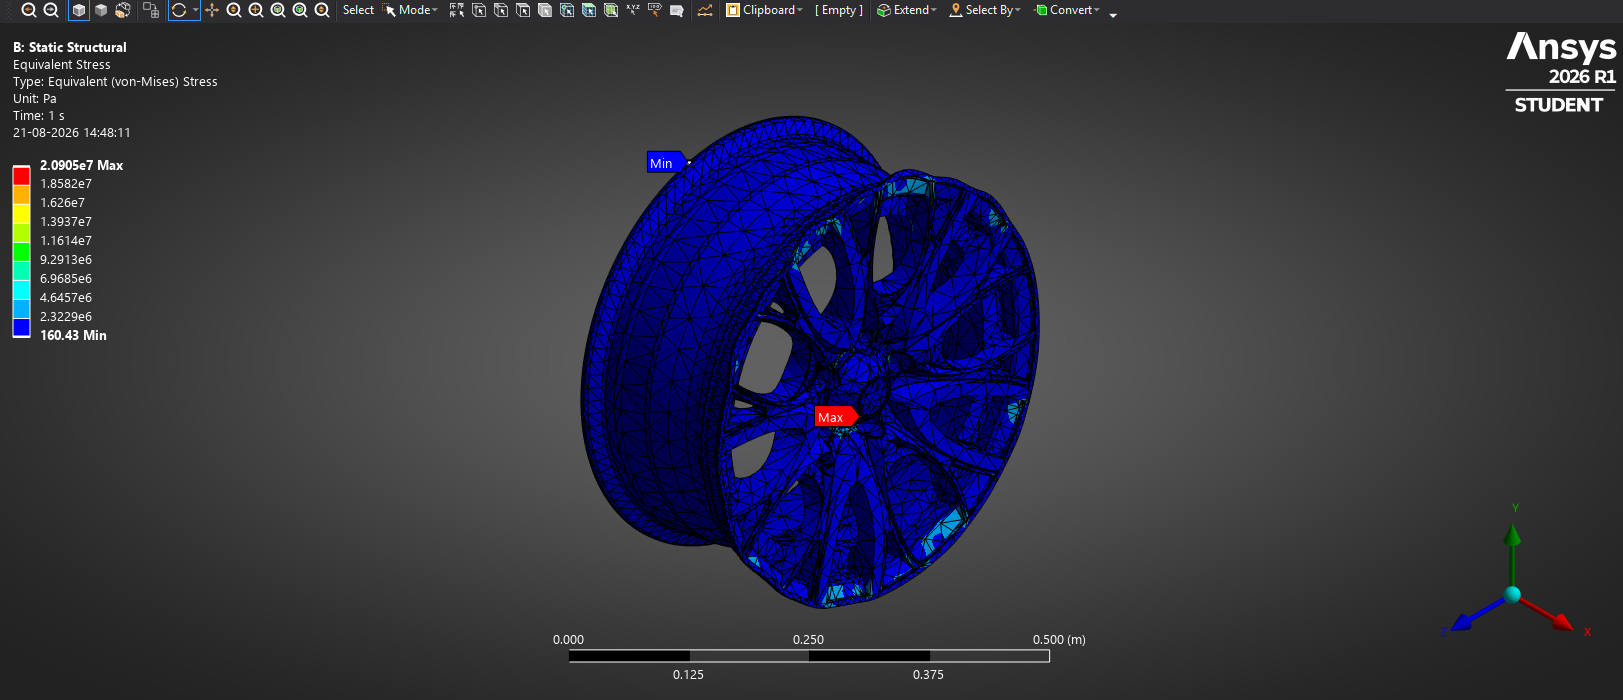
\includegraphics[width=\textwidth]{images/Static_Radial_Stress.png}
\caption{Equivalent (von-Mises) stress}
\end{subfigure}
\hfill
\begin{subfigure}{0.48\textwidth}
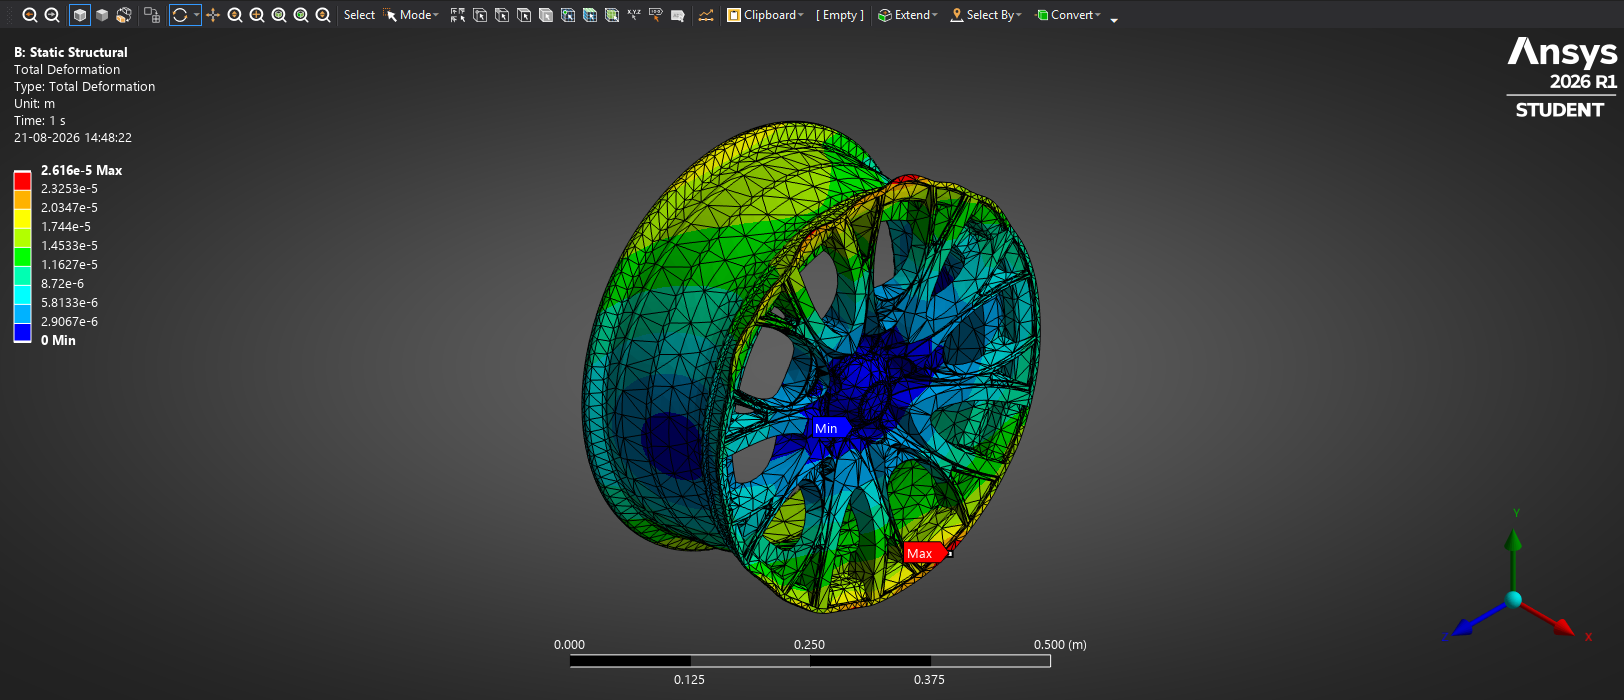
\includegraphics[width=\textwidth]{images/Static_Radial_Deformation.png}
\caption{Total deformation}
\end{subfigure}
\caption{Static structural results under the 4000~N radial load case.}
\label{fig:radial}
\end{figure}

\begin{figure}[H]
\centering
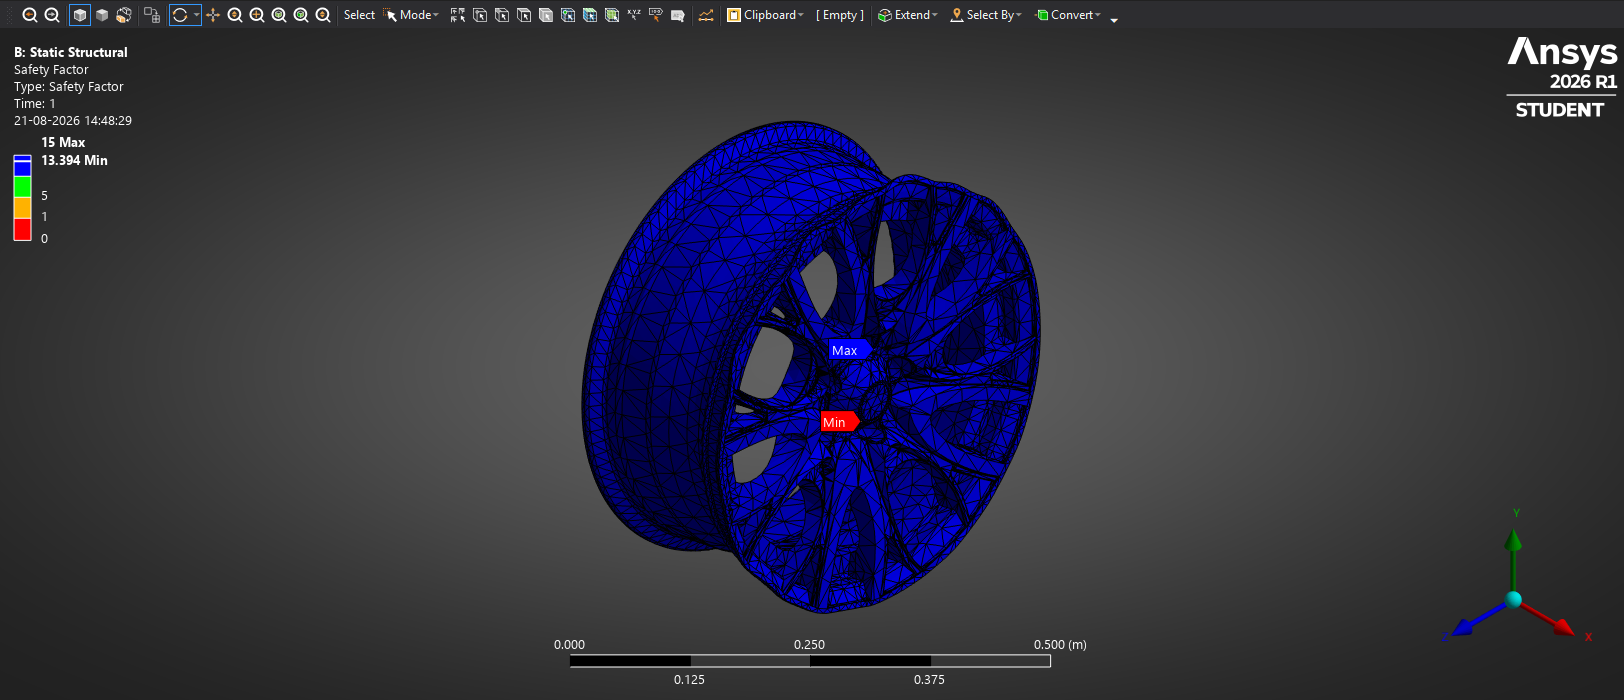
\includegraphics[width=0.55\textwidth]{images/Static_Radial_SafetyFactor.png}
\caption{Safety factor distribution under the radial load case (minimum SF = 13.4).}
\label{fig:radial_sf}
\end{figure}

Under this load, the wheel deflects by only $\sim$26~$\mu$m and reaches a maximum stress
of 20.9~MPa, far below the 280~MPa yield strength of the aluminium alloy. The resulting
safety factor of 13.4 indicates the design is very lightly stressed under a simple static
radial load -- as expected, since real wheels are rarely governed by this load case alone.

\subsection{Case 2: SAE J328 Bending Moment Results}

\begin{table}[H]
\centering
\caption{Static structural results under the 2000~N·m SAE J328 bending moment}
\label{tab:bending_results}
\begin{tabular}{lc}
\toprule
\textbf{Quantity} & \textbf{Value} \\
\midrule
Maximum Equivalent (von-Mises) Stress & 131.1 MPa \\
Maximum Total Deformation & 244.3 $\mu$m \\
Maximum Equivalent Elastic Strain & $1.86 \times 10^{-3}$ m/m \\
Minimum Safety Factor (vs. 280 MPa yield) & 2.1 \\
\bottomrule
\end{tabular}
\end{table}

\begin{figure}[H]
\centering
\begin{subfigure}{0.48\textwidth}
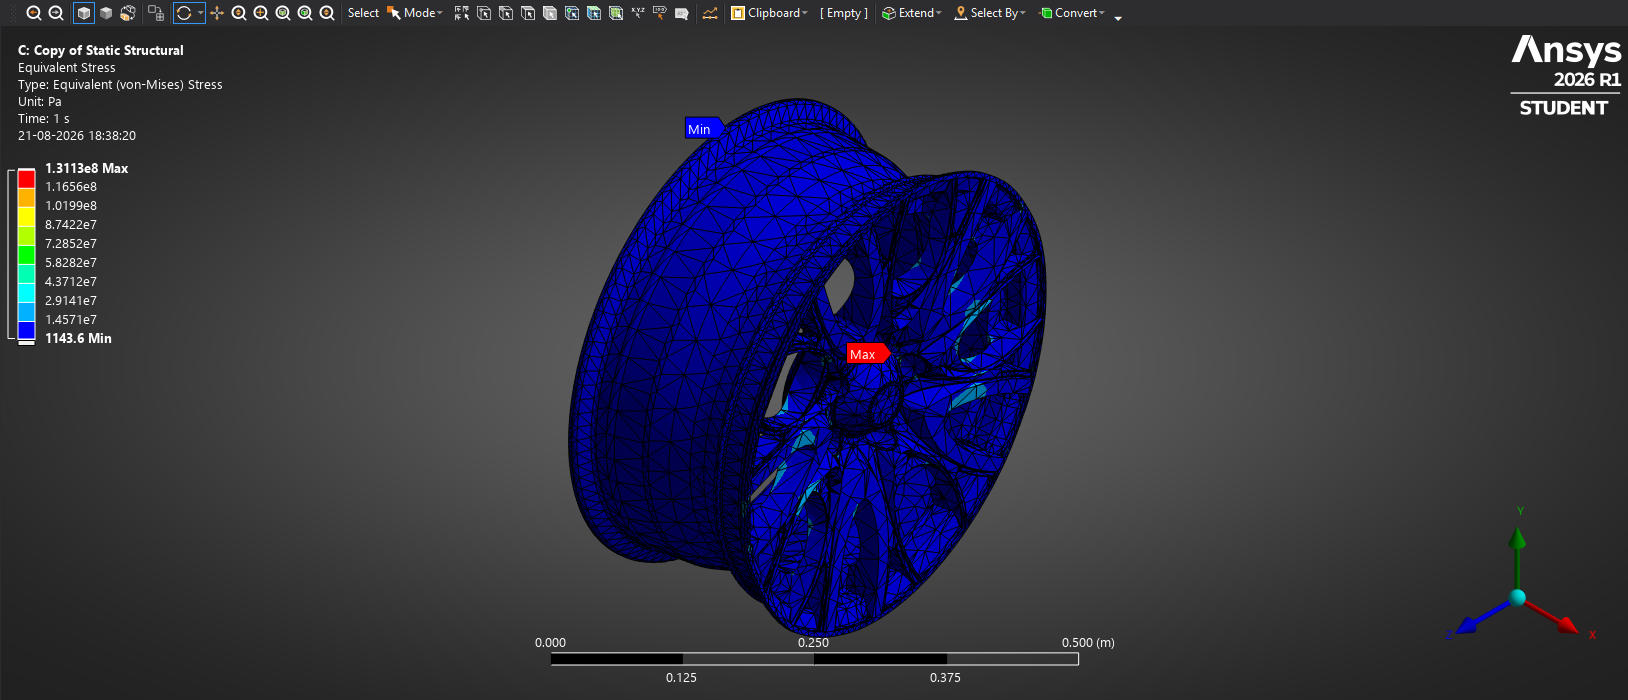
\includegraphics[width=\textwidth]{images/Static_Bending_Stress.png}
\caption{Equivalent (von-Mises) stress}
\end{subfigure}
\hfill
\begin{subfigure}{0.48\textwidth}
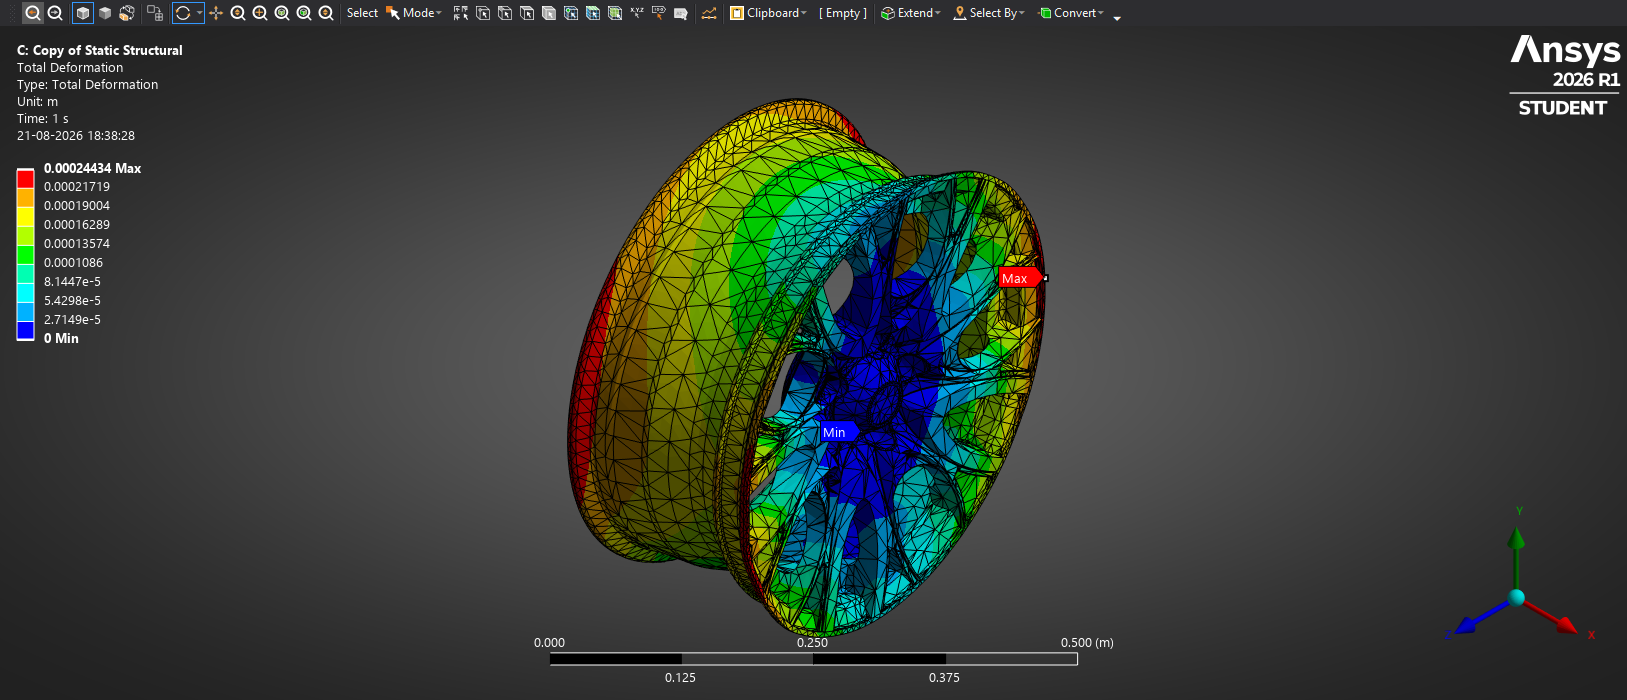
\includegraphics[width=\textwidth]{images/Static_Bending_Deformation.png}
\caption{Total deformation}
\end{subfigure}
\caption{Static structural results under the SAE J328 bending moment case.}
\label{fig:bending}
\end{figure}

\subsection{Comparison and Discussion}

\begin{table}[H]
\centering
\caption{Comparison of the two static load cases}
\label{tab:static_comparison}
\begin{tabular}{lccc}
\toprule
\textbf{Quantity} & \textbf{Radial (4000 N)} & \textbf{Bending (2000 N·m)} & \textbf{Ratio} \\
\midrule
Max. Equivalent Stress   & 20.9 MPa            & 131.1 MPa           & $\times 6.3$ \\
Max. Total Deformation   & 26.16 $\mu$m         & 244.3 $\mu$m         & $\times 9.3$ \\
Max. Equivalent Strain   & $2.96\times10^{-4}$  & $1.86\times10^{-3}$  & $\times 6.3$ \\
Minimum Safety Factor    & 13.4                 & 2.1                  & $\times 0.16$ \\
\bottomrule
\end{tabular}
\end{table}

The SAE J328 bending case produces roughly six to nine times higher stress, deformation,
and strain than the simplified radial load case, and reduces the safety factor from 13.4
down to 2.1. This is a substantial and physically meaningful difference, and illustrates
precisely why the automotive industry uses the rotating bending fatigue test, rather than
a simple static radial load, as the primary structural qualification test for wheels: the
bending case is the governing (more severe) load condition, and a safety factor of 13
under radial load alone would give a misleadingly optimistic impression of the design's
structural margin.

In both cases, the maximum stress is located near the spoke-to-hub transition on the
loaded side of the rim -- consistent with this region being the classical location where
bending load transitions from the spokes into the hub, and a commonly reported fatigue
crack initiation site in real wheel structures.

It is worth noting that a safety factor of 2.1 against yield under the SAE J328 static
case does not directly indicate the wheel's actual fatigue life, since the SAE J328 test
is fundamentally a cyclic (rotating) fatigue test; the static analysis performed here
captures only a single instant of that cycle and should be interpreted as a structural
stress check rather than a full fatigue-life prediction.

\subsection{Modelling Assumptions and Limitations (Static Analysis)}

\begin{itemize}
    \item The radial and bending loads are both applied as remote loads at a single point
    on the flange (representing the tire contact patch / loading arm location), rather
    than distributed over a realistic contact patch area.
    \item The bending moment magnitude uses standard SAE J328 formula inputs
    ($W = 4000$~N, $R = 0.30$~m, $\mu = 1.1$, $S = 1.5$); a specific vehicle's actual
    corner weight and tire radius would refine this value.
    \item The analysis is static, representing a single instant of the SAE J328 rotating
    bending cycle; a full fatigue-life assessment would require a rotating or cyclic
    loading simulation and S-N fatigue data for the material.
\end{itemize}

\begin{center}
{\LARGE\bfseries Part II}\\[0.3em]
{\Large\bfseries Modal Analysis}
\end{center}
\vspace{0.5em}

\section{Methodology}

All modal analyses were performed as linear eigenvalue analyses using the Block Lanczos
solver, extracting the first 12 modes in each case, using the same geometry, material,
and mesh described in Section~\ref{sec:geom}. Three boundary condition configurations
were studied:

\begin{itemize}
    \item \textbf{Free-Free:} no constraints applied. Used to validate the mass and
    stiffness properties of the model via the six expected rigid-body modes.
    \item \textbf{Constrained:} a Fixed Support applied to the cylindrical faces of the
    five bolt holes, representing the wheel bolted to a hub.
    \item \textbf{Tire-Loaded (Extension):} free-free baseline augmented with a
    Distributed Mass (10~kg total, representing the tire) applied to the outer flange
    face, and four longitudinal springs (50{,}000~N/m each, 200{,}000~N/m combined)
    connecting four symmetric points on the flange to fixed ground references, arranged
    at 90$^\circ$ intervals around the circumference to approximate distributed radial
    tire stiffness.
\end{itemize}

\section{Mesh Convergence Study}
\label{sec:convergence}
\label{sec:geom}

To ensure the reported natural frequencies were not dependent on mesh density, a
convergence study was performed on the free-free model by tracking the frequencies of
Mode~7 (first 2-nodal-diameter flange bending mode) and Mode~9 (first
3-nodal-diameter flange bending mode) across four mesh densities, ranging from the
default adaptive mesh down to a manually refined 0.0115~m element size (the practical
limit of the Ansys Student license used for this project).

\begin{table}[H]
\centering
\caption{Mesh convergence results for Mode 7 and Mode 9}
\label{tab:convergence}
\begin{tabular}{lccc}
\toprule
\textbf{Element Size (m)} & \textbf{Nodes} & \textbf{Mode 7 (Hz)} & \textbf{Mode 9 (Hz)} \\
\midrule
0.0345 (default/adaptive) & 54{,}523  & 385.79 & 780.39 \\
0.0150 (coarse)           & 88{,}409  & 382.28 & 773.17 \\
0.0120 (medium)           & 111{,}762 & 381.47 & 772.00 \\
0.0115 (fine)             & 116{,}074 & 381.37 & 771.76 \\
\bottomrule
\end{tabular}
\end{table}

\begin{figure}[H]
\centering
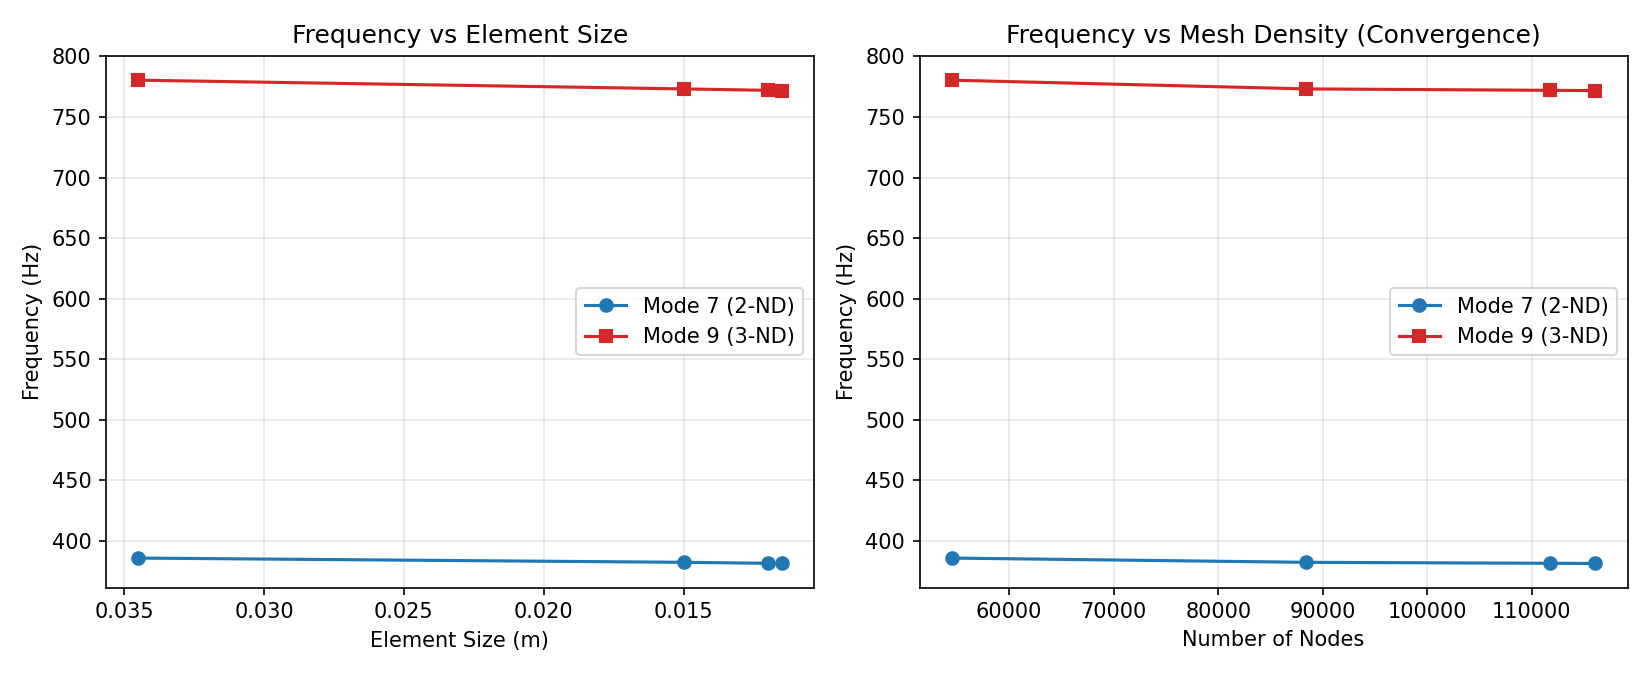
\includegraphics[width=0.95\textwidth]{images/convergence_plot.png}
\caption{Convergence of Mode 7 and Mode 9 frequencies with element size (left) and node
count (right).}
\label{fig:convergence}
\end{figure}

Between the medium (0.012~m) and fine (0.0115~m) meshes, Mode~7 changed by only
0.10~Hz and Mode~9 by only 0.24~Hz -- both well under 0.1\% -- indicating that the
solution is effectively mesh-independent at this density. All modal results in this
report are reported using this converged 0.0115~m mesh. This same converged mesh density
was also used for both static structural load cases in Part~I.

\section{Free-Free Modal Analysis}

\subsection{Overview}

The free-free configuration (no boundary conditions) was used first, both as a
baseline for comparison and as a validation check: a correctly modelled free-free
structure must exhibit exactly six rigid-body modes (three translational, three
rotational) at approximately 0~Hz, before any flexible (deformable) modes appear.

\begin{table}[H]
\centering
\caption{Free-free modal analysis results (converged mesh, 0.0115~m)}
\label{tab:freefree}
\begin{tabular}{clc}
\toprule
\textbf{Mode(s)} & \textbf{Description} & \textbf{Frequency (Hz)} \\
\midrule
1 -- 6  & Rigid body modes (translation + rotation) & $\approx 0$ \\
7 -- 8  & 2-nodal-diameter flange bending (degenerate pair) & 381.37 / 381.38 \\
9 -- 10 & 3-nodal-diameter flange bending (degenerate pair) & 771.76 / 771.80 \\
11      & Axisymmetric ``umbrella'' (axial breathing) mode & 1171.34 \\
12      & 4-nodal-diameter flange bending & 1249.79 \\
\bottomrule
\end{tabular}
\end{table}

\subsection{Discussion of Mode Shapes}

Modes 1 through 6 were confirmed to occur at (numerically) zero frequency, verifying
the correctness of the model's mass and inertia properties and the absence of any
unintended constraints.

The first flexible modes (7--8) form a closely spaced pair at $\approx 381$~Hz, each
showing a two-lobe (2-nodal-diameter) bending pattern concentrated in the outer flange,
with the spokes and hub remaining comparatively rigid (Figure~\ref{fig:ff7}). The close
frequency spacing between the pair is characteristic of near-axisymmetric structures,
where the same physical mode shape can occur in two orthogonal circumferential
orientations.

Modes 9--10 (Figure~\ref{fig:ff9}) follow the same pattern but with a
3-nodal-diameter shape, again as a closely spaced degenerate pair, at $\approx
772$~Hz -- consistent with the classical trend in disc/ring vibration theory, where
increasing the number of nodal diameters increases the modal stiffness and hence the
frequency.

Mode 11 (Figure~\ref{fig:ff11}) breaks from this pattern: rather than
concentrated flange bending, the entire disc face -- spokes and hub together -- moves
axially in a roughly axisymmetric ``umbrella'' or breathing pattern. This is a
physically distinct mode family governed primarily by spoke bending stiffness, rather
than flange bending stiffness, and its appearance between the 3-ND and 4-ND flange
modes (rather than after them) illustrates that mode number does not necessarily
correspond to increasing shape complexity -- different structural mechanisms can
interleave in frequency depending on the specific geometry.

Mode 12 (1249.79~Hz, not shown separately) returns to the flange-bending family,
showing a clear 4-nodal-diameter pattern similar to Modes 7--10 but with one
additional lobe.

\begin{figure}[H]
\centering
\begin{subfigure}{0.48\textwidth}
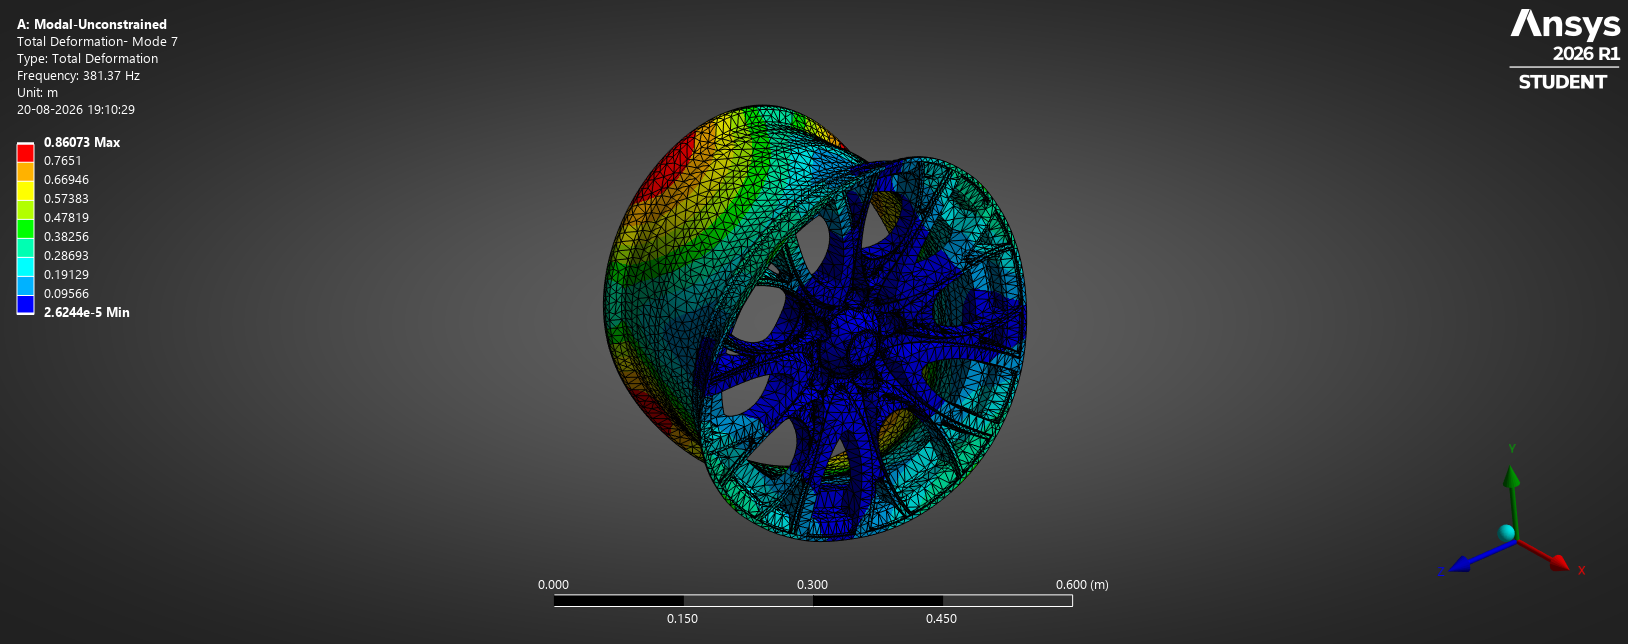
\includegraphics[width=\textwidth]{images/Modal_Unconstrained_7.png}
\caption{Mode 7, 381.37 Hz -- 2-ND flange bending}
\label{fig:ff7}
\end{subfigure}
\hfill
\begin{subfigure}{0.48\textwidth}
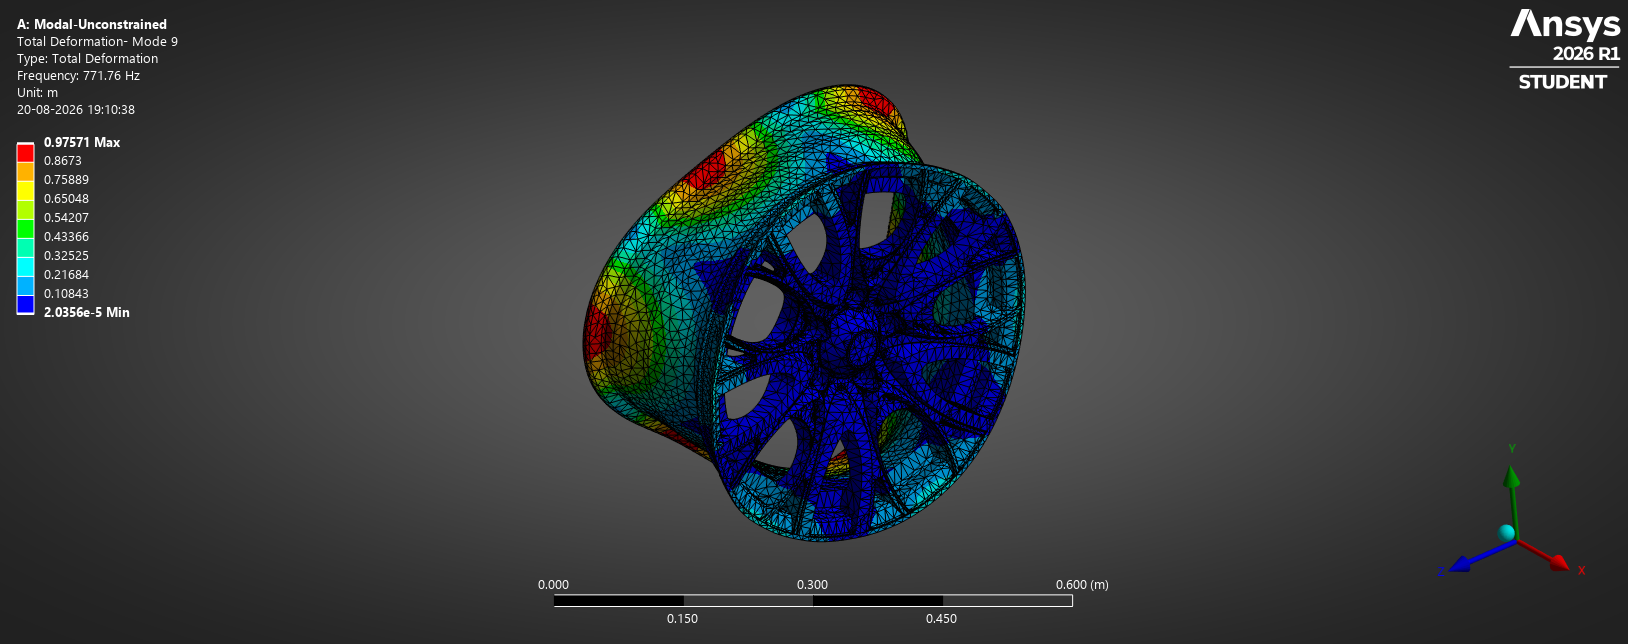
\includegraphics[width=\textwidth]{images/Modal_Unconstrained_9.png}
\caption{Mode 9, 771.76 Hz -- 3-ND flange bending}
\label{fig:ff9}
\end{subfigure}
\caption{Free-free flange bending mode shapes.}
\end{figure}

\begin{figure}[H]
\centering
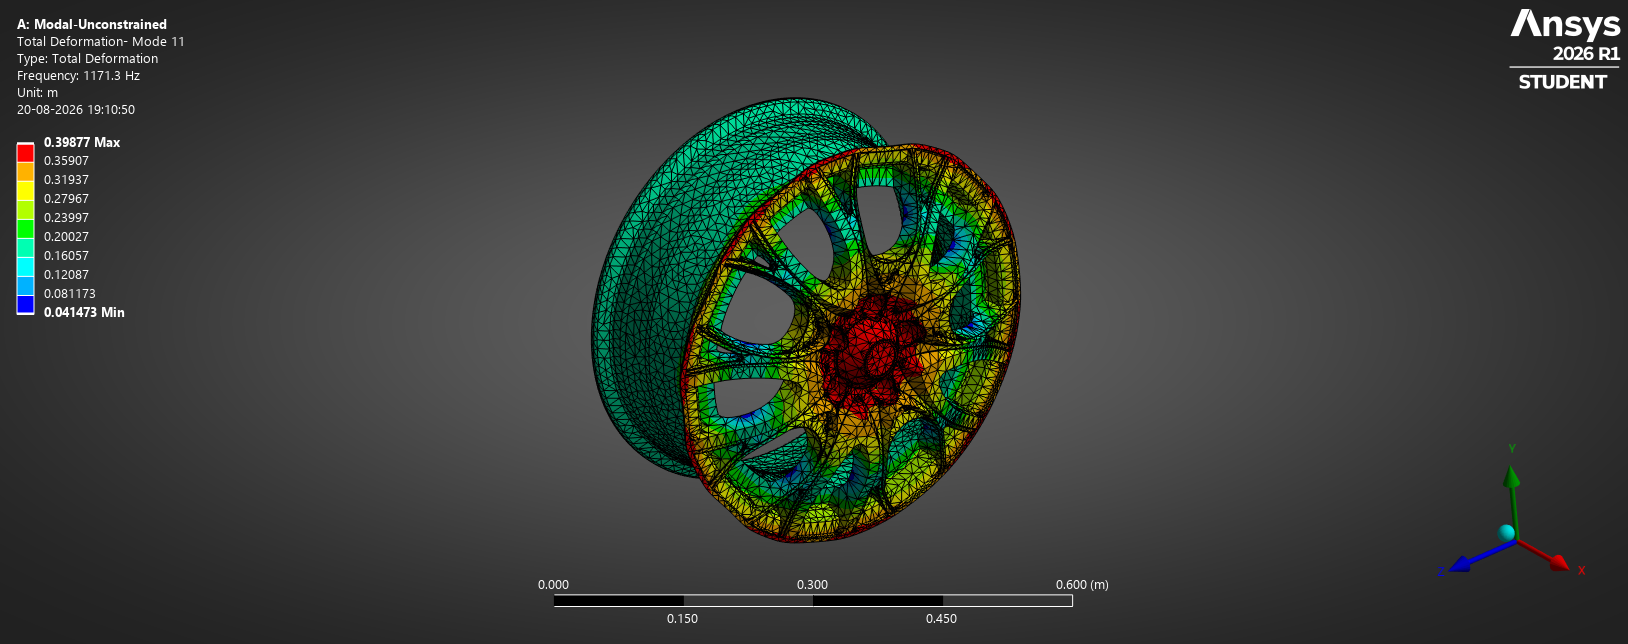
\includegraphics[width=0.55\textwidth]{images/Modal_Unconstrained_11.png}
\caption{Mode 11, 1171.34 Hz -- axisymmetric umbrella (axial breathing) mode.}
\label{fig:ff11}
\end{figure}

\section{Constrained Modal Analysis}

\subsection{Overview}

To represent a realistic mounting condition, a Fixed Support boundary condition was
applied to the cylindrical faces of the five bolt holes. Under this constraint, the six
rigid-body modes are eliminated entirely, and the lowest-frequency mode becomes a
genuine flexible mode.

\begin{table}[H]
\centering
\caption{Constrained modal analysis results (bolt-hole fixed support)}
\label{tab:constrained}
\begin{tabular}{clc}
\toprule
\textbf{Mode(s)} & \textbf{Description} & \textbf{Frequency (Hz)} \\
\midrule
1 -- 2   & Axisymmetric ring mode (low order) & 390.02 / 390.22 \\
3 -- 4   & 2-nodal-diameter flange bending & 433.72 / 443.72 \\
5 -- 6   & Spoke-bending dominated mode & 679.96 / 699.26 \\
7 -- 8   & 3-nodal-diameter flange bending & 780.50 / 780.55 \\
9, 11    & 4-nodal-diameter flange bending & 1264.62 / 1274.63 \\
\bottomrule
\end{tabular}
\end{table}

\subsection{Comparison with Free-Free Results}

\begin{table}[H]
\centering
\caption{Frequency comparison between free-free and constrained configurations, grouped
by physical mode family}
\label{tab:comparison}
\begin{tabular}{lcc}
\toprule
\textbf{Mode Family} & \textbf{Free-Free (Hz)} & \textbf{Constrained (Hz)} \\
\midrule
Rigid body                     & $\approx 0$        & --- (eliminated) \\
Axisymmetric ring (low order)  & ---                 & 390.02 -- 390.22 \\
2-ND flange bending            & 381.37 -- 381.38    & 433.72 -- 443.72 \\
Spoke-bending                  & ---                 & 679.96 -- 699.26 \\
3-ND flange bending            & 771.76 -- 771.80    & 780.50 -- 780.55 \\
Umbrella (axial breathing)     & 1171.34              & --- (not isolated) \\
4-ND flange bending            & 1249.79              & 1264.62 -- 1274.63 \\
\bottomrule
\end{tabular}
\end{table}

\subsection{Discussion}

Fixing the hub via the bolt holes produces two important effects, clearly visible in
Table~\ref{tab:comparison}:

\textbf{New mode families appear.} The axisymmetric ring mode (modes 1--2,
$\approx 390$~Hz) and the spoke-bending mode (modes 5--6, $\approx 680$--$700$~Hz)
did not exist in the free-free case. In the free-free model, this type of motion is
mathematically indistinguishable from rigid-body translation/rotation and is absorbed
into the zero-frequency rigid body modes; once the hub is fixed, these become genuine,
distinguishable flexible modes with real, non-zero frequencies.

\textbf{Higher-order flange modes are largely insensitive to the hub constraint.} The
3-nodal-diameter mode shifts by less than 0.2~Hz (771.8~$\rightarrow$~780.5~Hz) --
essentially unchanged -- while the 2-nodal-diameter mode shifts substantially
(381.4~$\rightarrow$~$\sim$438~Hz, an increase of roughly 15\%). Mode shape
visualisation (Figures~\ref{fig:c1}--\ref{fig:c9}) shows that the higher-order flange
modes have their maximum deformation concentrated in the outer flange, with very little
motion at the hub; consequently, constraining the hub has little effect on their
frequency. The 2-ND mode, by contrast, involves more participation from the hub/spoke
region and is therefore more sensitive to how that region is supported.

\begin{figure}[H]
\centering
\begin{subfigure}{0.48\textwidth}
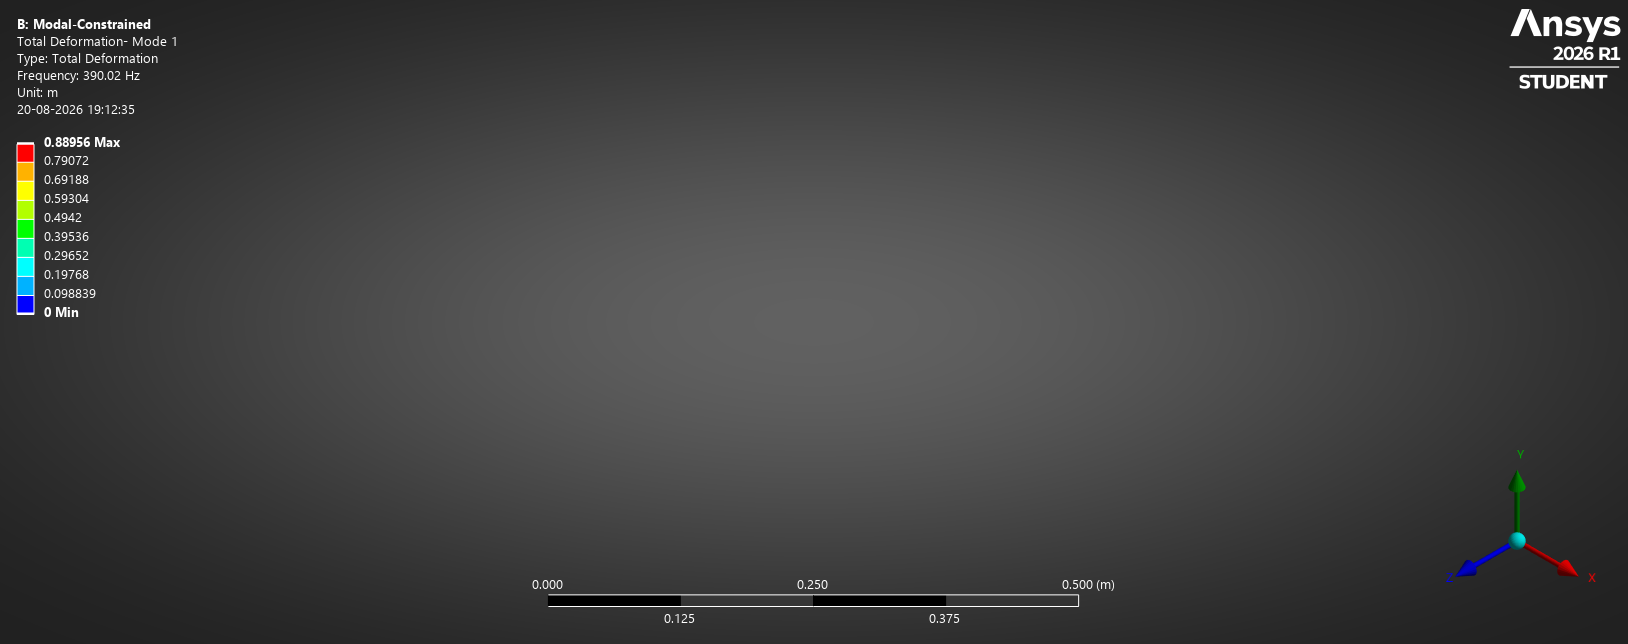
\includegraphics[width=\textwidth]{images/Modal_Constrained_1.png}
\caption{Mode 1, 390.02 Hz -- axisymmetric ring mode}
\label{fig:c1}
\end{subfigure}
\hfill
\begin{subfigure}{0.48\textwidth}
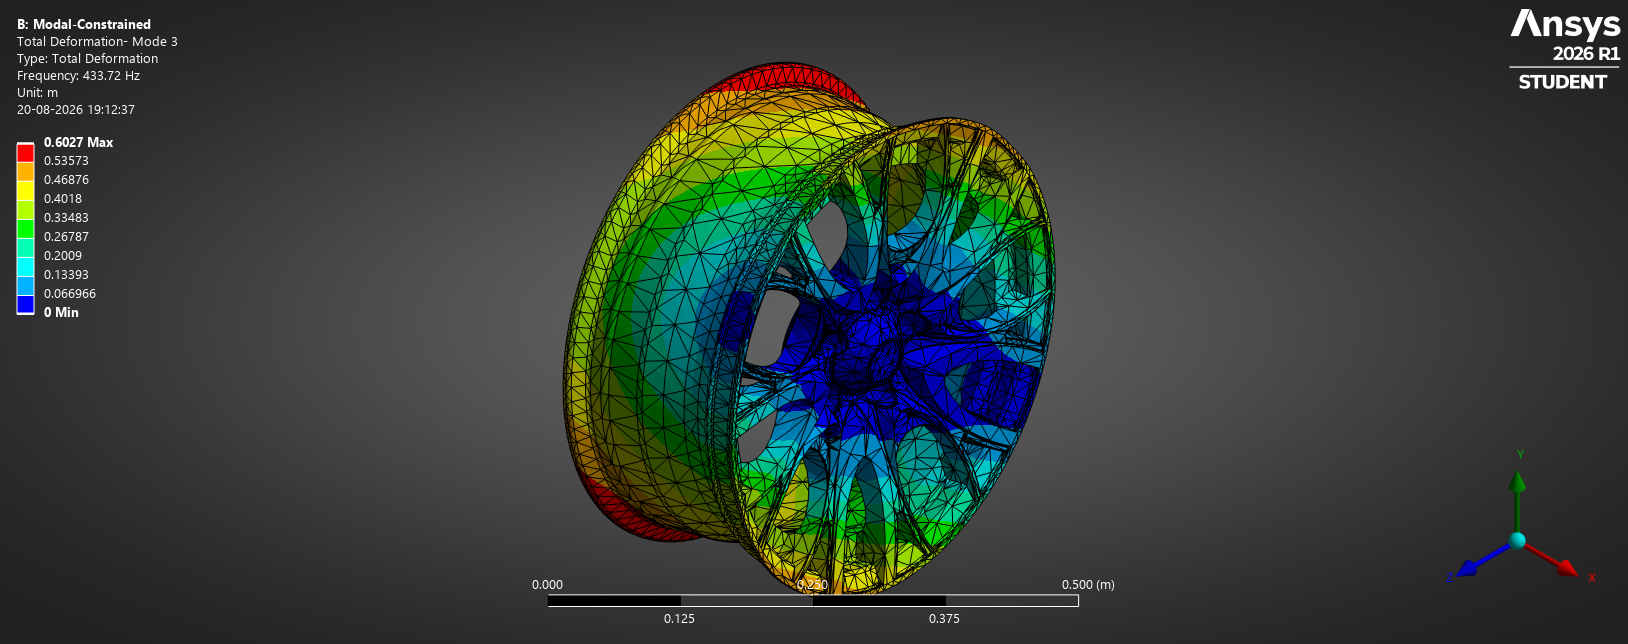
\includegraphics[width=\textwidth]{images/Modal_Constrained_3.png}
\caption{Mode 3, 433.72 Hz -- 2-ND flange bending}
\label{fig:c3}
\end{subfigure}
\caption{Constrained low-order mode shapes.}
\end{figure}

\begin{figure}[H]
\centering
\begin{subfigure}{0.48\textwidth}
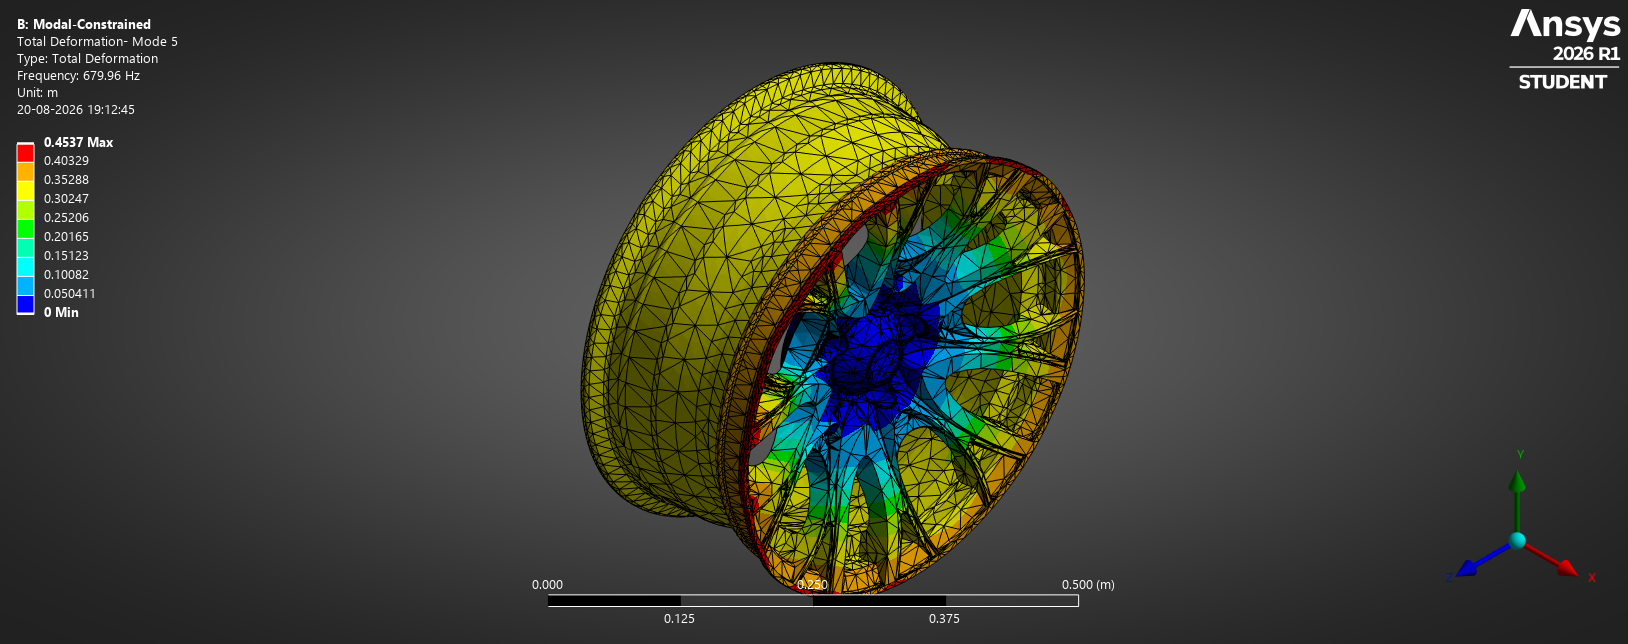
\includegraphics[width=\textwidth]{images/Modal_Constrained_5.png}
\caption{Mode 5, 679.96 Hz -- spoke-bending mode}
\label{fig:c5}
\end{subfigure}
\hfill
\begin{subfigure}{0.48\textwidth}
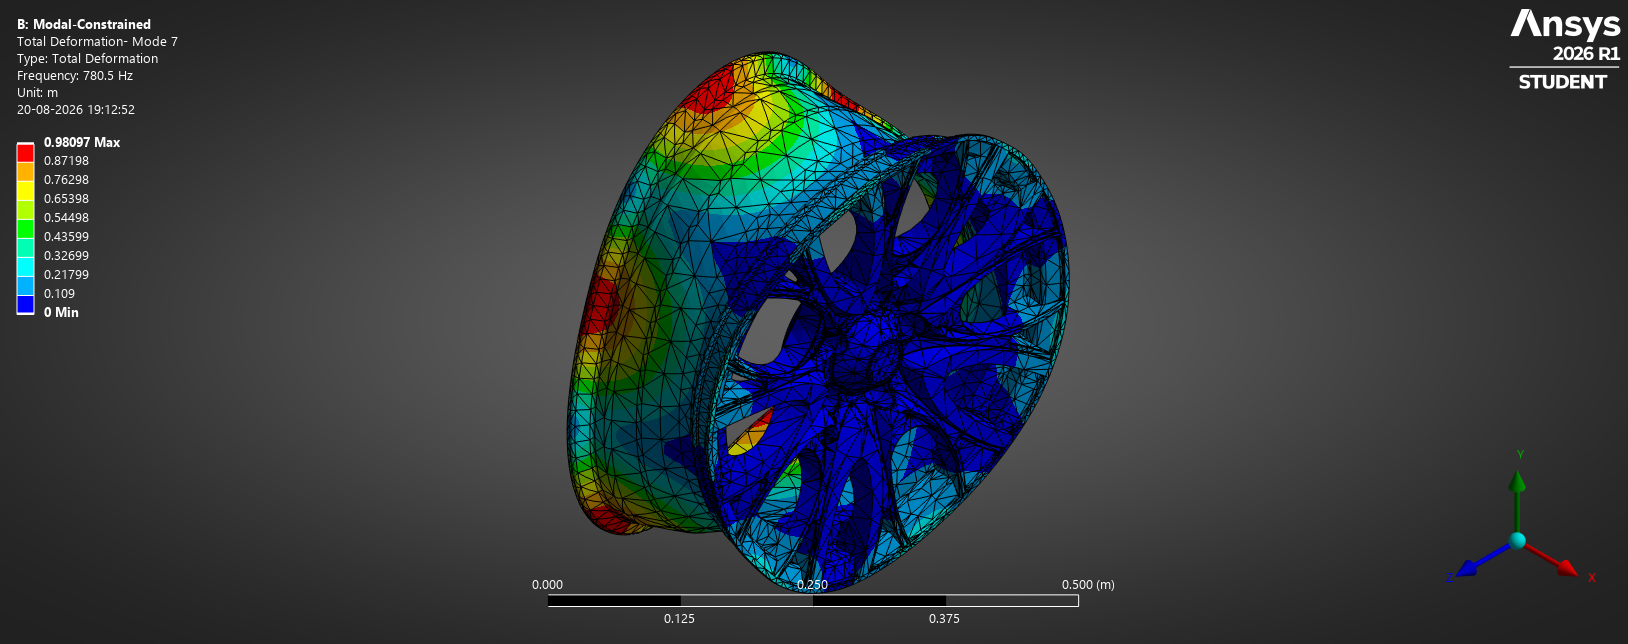
\includegraphics[width=\textwidth]{images/Modal_Constrained_7.png}
\caption{Mode 7, 780.50 Hz -- 3-ND flange bending (unchanged from free-free)}
\label{fig:c7}
\end{subfigure}
\caption{Constrained spoke-bending and 3-ND flange modes.}
\end{figure}

\begin{figure}[H]
\centering
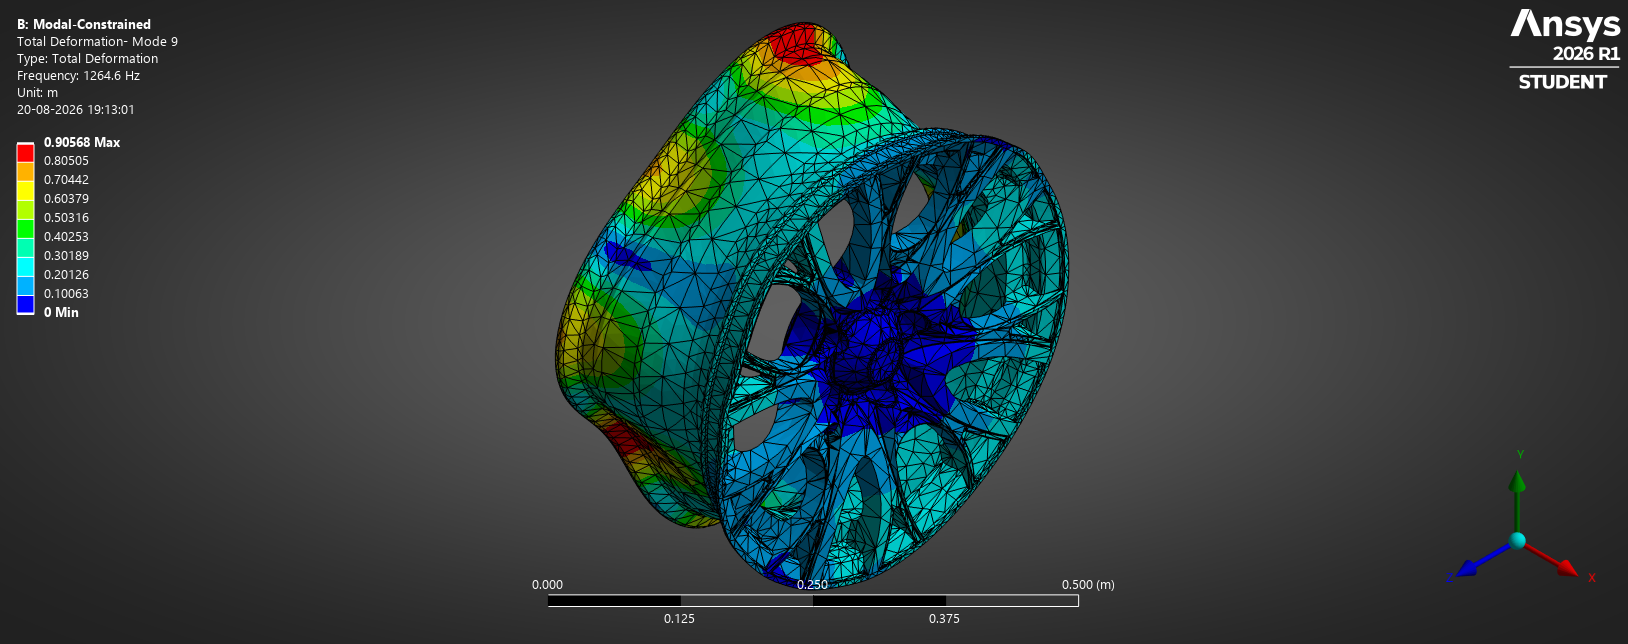
\includegraphics[width=0.5\textwidth]{images/Modal_Constrained_9.png}
\caption{Mode 9, 1264.62 Hz -- 4-ND flange bending (constrained).}
\label{fig:c9}
\end{figure}

\section{Tire-Loaded Extension}

\subsection{Modelling Approach}

As an extension to the free-free study, the effect of a mounted tire was approximated
using a simplified lumped model:

\begin{itemize}
    \item \textbf{Tire mass:} modelled as a Distributed Mass of 10~kg, scoped to the
    entire outer flange face, so that mass loading is spread continuously around the
    circumference rather than concentrated at discrete points.
    \item \textbf{Tire stiffness:} modelled as four longitudinal (radial) springs, each
    of stiffness 50{,}000~N/m (200{,}000~N/m combined), connecting four points on the
    flange -- spaced at 90$^\circ$ intervals around the circumference -- to fixed ground
    references along the corresponding radial directions.
\end{itemize}

An initial attempt using four discrete point masses (2.5~kg each) at the same four
locations, rather than a distributed mass, was found to have almost no effect on the
flange bending mode frequencies. This is because the point masses did not align with
the regions of maximum modal displacement around the full circumference, and so did
not meaningfully couple with the flexible mode shapes. Switching to a distributed mass
produced substantial, physically meaningful frequency shifts, illustrating that the
spatial distribution of an approximated mass or stiffness element -- not just its total
magnitude -- is critical to obtaining a representative simplified model.

\subsection{Results}

\begin{table}[H]
\centering
\caption{Tire-loaded modal analysis results (distributed mass + 4 springs)}
\label{tab:tire}
\begin{tabular}{clcc}
\toprule
\textbf{Mode(s)} & \textbf{Description} & \textbf{Frequency (Hz)} & \textbf{vs. Free-Free} \\
\midrule
1 -- 4  & Residual rigid body & $\approx 0$ & -- \\
5 -- 6  & Rigid-body ``bounce'' mode on tire springs & 20.84 / 20.84 & new \\
7 -- 8  & 2-ND flange bending & 283.77 / 283.95 & $-25.6\%$ \\
9 -- 10 & 3-ND flange bending & 613.18 / 613.21 & $-20.6\%$ \\
11      & Axisymmetric umbrella mode & 764.58 & $-34.7\%$ \\
12      & 4-ND flange bending & 838.87 & $-32.9\%$ \\
\bottomrule
\end{tabular}
\end{table}

\subsection{Discussion}

Two new low-frequency modes (5--6, $\approx 20.8$~Hz) appear once the tire springs
are introduced. Mode-shape animation (Figure~\ref{fig:t5}) shows the entire rim
translating almost rigidly against the four tire springs, with very little internal
flexing -- analogous to the classical ``wheel hop'' or unsprung-mass bounce mode
familiar from vehicle dynamics, and a reassuring qualitative validation that the
simplified spring model captures the expected low-frequency behaviour of a
tire-mounted wheel.

All of the higher flexible modes shift down substantially once the tire's mass is
included (Table~\ref{tab:tire}), by 21--35\%. This is consistent with $\omega \propto
\sqrt{k/m}$: adding participating mass around the flange, where these modes already
have their largest displacement, reduces their natural frequency without requiring any
change in the underlying structural stiffness. The umbrella mode (mode 11) shows the
largest relative shift, suggesting its axisymmetric, largely axial motion couples
particularly strongly with the added radial-mass distribution at the flange.

\begin{figure}[H]
\centering
\begin{subfigure}{0.48\textwidth}
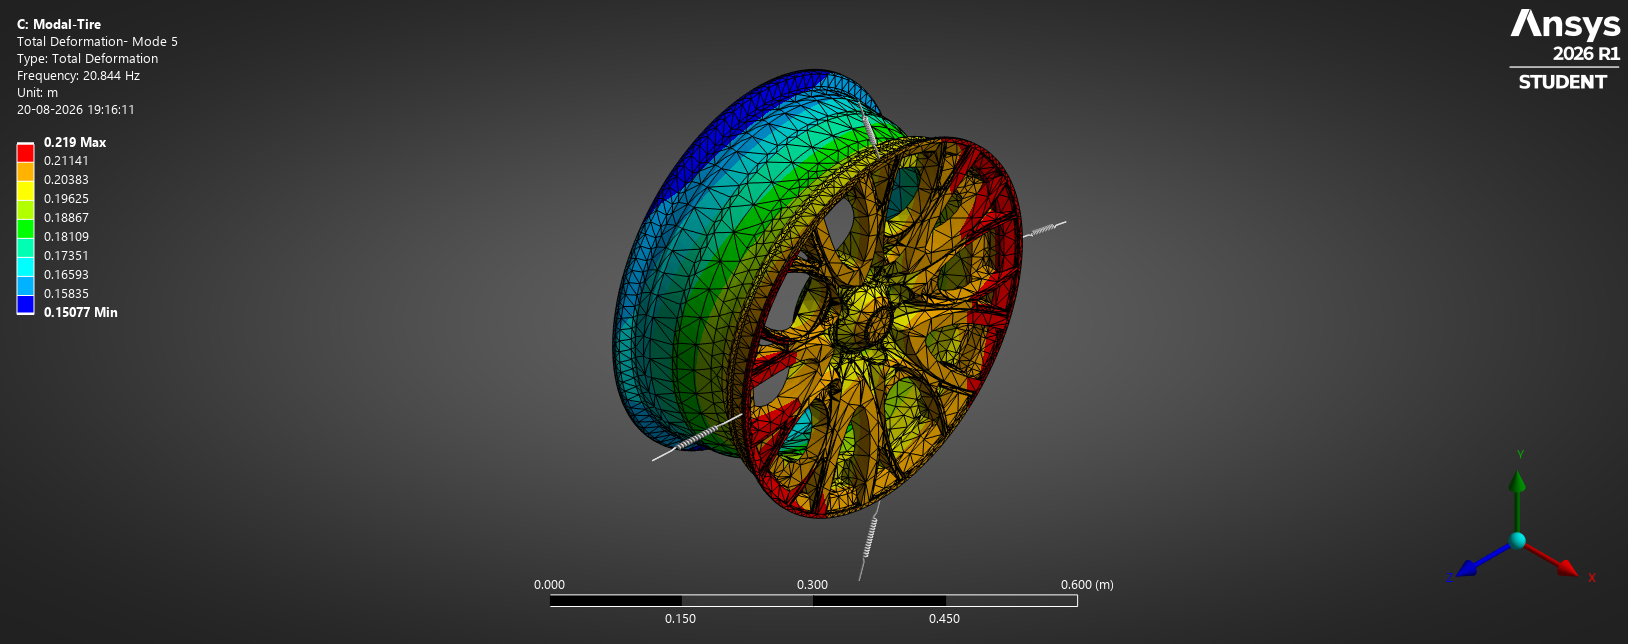
\includegraphics[width=\textwidth]{images/Tire-Mode5.png}
\caption{Mode 5, 20.84 Hz -- rigid-body bounce mode}
\label{fig:t5}
\end{subfigure}
\hfill
\begin{subfigure}{0.48\textwidth}
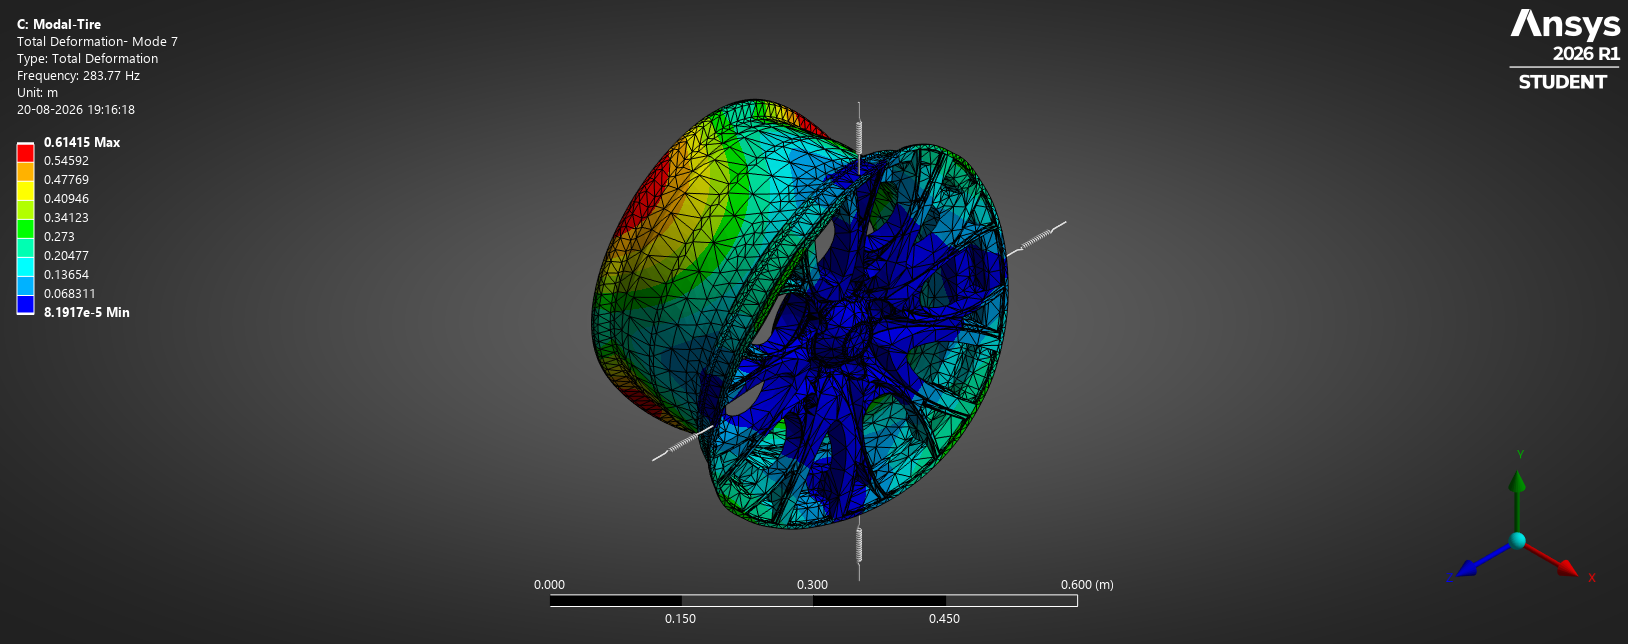
\includegraphics[width=\textwidth]{images/Tire-Mode7.png}
\caption{Mode 7, 283.77 Hz -- 2-ND flange bending (mass-loaded)}
\label{fig:t7}
\end{subfigure}
\caption{Tire-loaded mode shapes: bounce mode and mass-loaded 2-ND flange mode.}
\end{figure}

\begin{figure}[H]
\centering
\begin{subfigure}{0.48\textwidth}
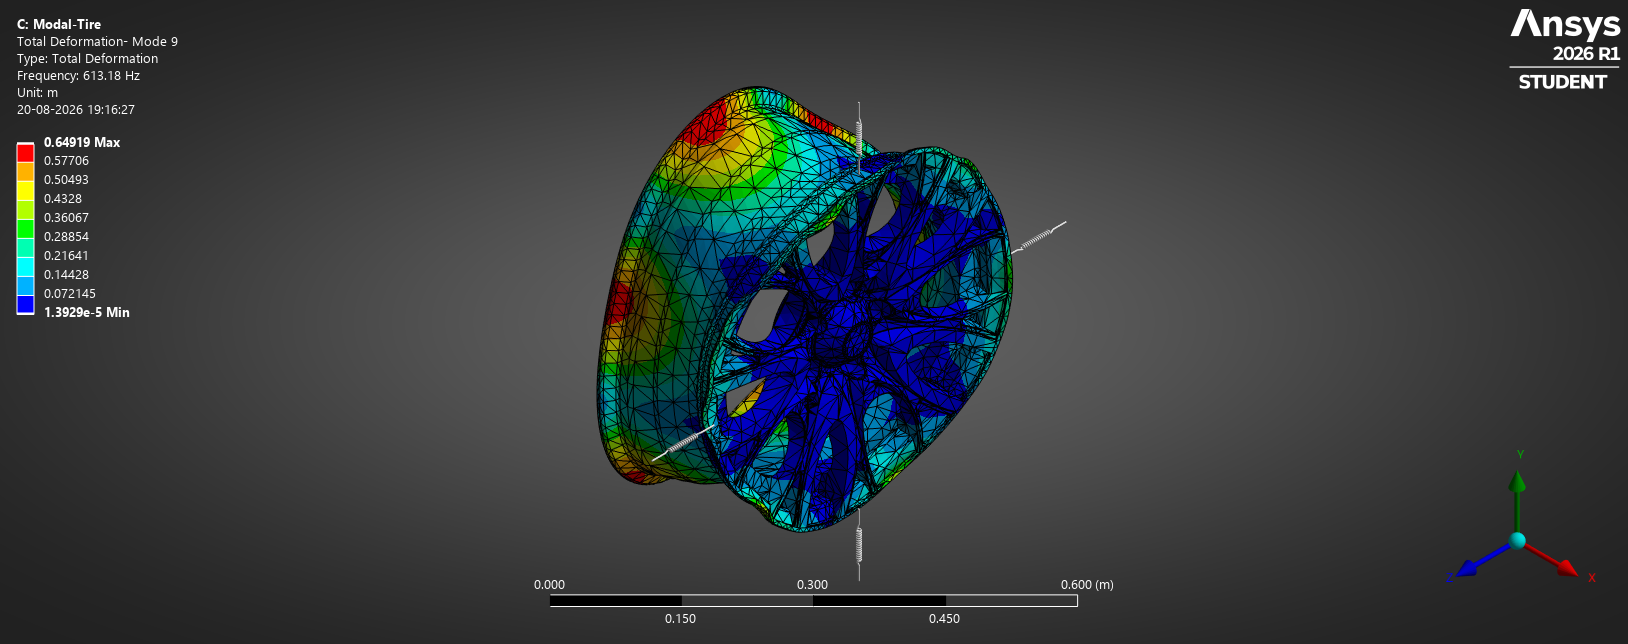
\includegraphics[width=\textwidth]{images/Tire-Mode9.png}
\caption{Mode 9, 613.18 Hz -- 3-ND flange bending (mass-loaded)}
\label{fig:t9}
\end{subfigure}
\hfill
\begin{subfigure}{0.48\textwidth}
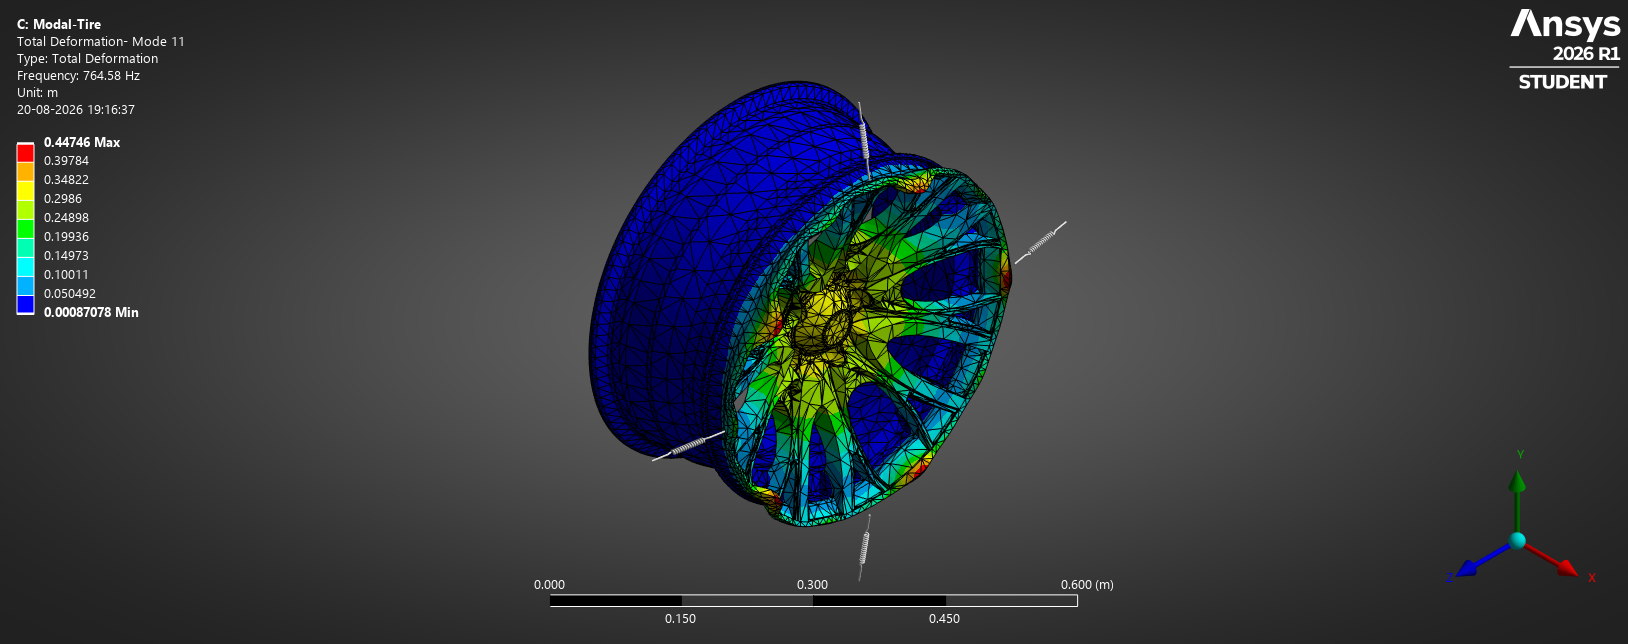
\includegraphics[width=\textwidth]{images/Tire-Mode11.png}
\caption{Mode 11, 764.58 Hz -- umbrella mode (mass-loaded)}
\label{fig:t11}
\end{subfigure}
\caption{Tire-loaded higher-order flange and umbrella mode shapes.}
\end{figure}

\subsection{Modelling Limitations}

The tire-loaded model presented here is a first-order approximation intended to
illustrate the qualitative effect of tire mass and stiffness, and has several known
limitations worth noting:

\begin{itemize}
    \item Tire stiffness is lumped at four discrete circumferential locations (though
    mass is distributed continuously); a fully distributed spring-mass ring, or a full
    3-D tire model with contact, would give a more accurate representation.
    \item The assumed tire mass (10~kg) and combined radial stiffness
    (200{,}000~N/m) are representative estimates for a passenger car tire, not measured
    values for a specific tire.
    \item Only the free-free baseline was extended with the tire model; a combined
    constrained-plus-tire case (representing the fully mounted, tire-loaded wheel) was
    not analysed but would be a natural next step.
\end{itemize}

\section{Overall Conclusions}

This project combined a static structural assessment and a modal characterisation of a
SolidWorks-modelled multi-spoke wheel rim in Ansys Mechanical. The key findings are
summarised below.

\subsection{Static Structural Analysis}

\begin{enumerate}
    \item Under a simplified 4000~N radial load, the wheel is very lightly stressed
    (max. 20.9~MPa, safety factor 13.4), indicating that a simple static radial load is
    not the governing design case for this component.
    \item Under the SAE J328 cornering bending moment (2000~N·m), stress,
    deformation, and strain all increase by roughly 6--9$\times$ relative to the radial
    case, and the safety factor drops to 2.1 -- confirming that the industry-standard
    bending fatigue test represents a substantially more severe and structurally
    meaningful loading condition than a simple radial load.
    \item In both load cases, maximum stress concentrates at the spoke-to-hub
    transition, consistent with commonly reported fatigue crack initiation sites in
    real wheel structures.
\end{enumerate}

\subsection{Modal Analysis}

\begin{enumerate}
    \item A mesh convergence study confirmed that a 0.0115~m element size
    (116{,}074 nodes) produces mesh-independent frequencies for the modes of interest,
    with less than 0.3~Hz change between the two finest meshes studied.
    \item The free-free model correctly exhibited six near-zero-frequency rigid body
    modes, followed by a clear progression of flange-bending modes (2-ND at 381~Hz,
    3-ND at 772~Hz, 4-ND at 1250~Hz) and a distinct axisymmetric umbrella mode at
    1171~Hz, validating the model's mass and stiffness distribution.
    \item Constraining the bolt holes eliminates the rigid-body modes and introduces
    two new mode families (an axisymmetric ring mode and a spoke-bending mode) not
    distinguishable in the free-free case, while higher-order flange bending modes
    remain largely insensitive to the hub boundary condition.
    \item A simplified tire model (distributed mass + four radial springs) introduced
    a new low-frequency ``bounce'' mode and reduced all higher flexible mode
    frequencies by 21--35\%, with the spatial distribution of the approximated mass
    proving far more influential than its total value alone.
\end{enumerate}

\section*{Appendix: Assumptions Summary}
\addcontentsline{toc}{section}{Appendix: Assumptions Summary}

\begin{table}[H]
\centering
\caption{Summary of key modelling assumptions}
\begin{tabular}{ll}
\toprule
\textbf{Assumption} & \textbf{Value} \\
\midrule
Material & Aluminium alloy (356.0-T6 cast, $\rho=2770$ kg/m$^3$) \\
Mesh (final, converged) & 0.0115 m element size, 116{,}074 nodes \\
Modal solver & Block Lanczos, 12 modes extracted \\
Constrained BC (modal \& static) & Fixed support on 5 bolt-hole cylindrical faces \\
Radial load & 4000 N, applied at flange contact point \\
SAE J328 bending moment & 2000 N·m ($W$=4000 N, $R$=0.30 m, $\mu$=1.1, $S$=1.5) \\
Tire mass (modal extension) & 10 kg, distributed over outer flange face \\
Tire radial stiffness (modal ext.) & 200{,}000 N/m total (4 $\times$ 50{,}000 N/m springs) \\
\bottomrule
\end{tabular}
\end{table}

\end{document}
